\documentclass[11pt]{article}
% --- Encoding e font ---
\usepackage[utf8]{inputenc}
\usepackage[T1]{fontenc}
\usepackage{lmodern}

% --- Matematica ---
\usepackage{amsmath,amssymb,amsfonts,gensymb,amsthm}
\DeclareMathOperator*{\argmin}{arg\,min}
\DeclareMathOperator*{\argmax}{arg\,max}
\usepackage{centernot}
% --- Grafica, colori, float ---
\usepackage{graphicx}
\usepackage[dvipsnames]{xcolor}
\usepackage{float}
% --- Liste e ambienti ---
\usepackage{enumitem}
% --- Caption, numerazione figure ---
\usepackage{caption}
\usepackage{chngcntr}
% --- Caption, numerazione figure ---
\captionsetup{font=small, labelfont=bf, textfont=it}
% --- Indice/TOC personalizzazione (se ti serve) ---
\usepackage{tocloft}
% --- colorbox
\usepackage[most]{tcolorbox}
%--- spazio tra le riga
\usepackage{parskip}
\setlength{\parskip}{0.15cm}
% Elenchi compatti:
\setlist[itemize]{ topsep=2pt, itemsep=0pt, parsep=0pt}
\setlist[enumerate]{topsep=2pt, itemsep=0pt, parsep=0pt}

% Per il codice
\usepackage{listings}
% Definisci i colori esatti di VS Code (tema Light+)
\definecolor{vscodeblue}{RGB}{0,0,255}          % Keywords
\definecolor{vscodeorange}{RGB}{163,21,21}      % Strings
\definecolor{vscodegreen}{RGB}{0,128,0}         % Comments
\definecolor{vscodepurple}{RGB}{197,134,192}    % Control flow e import
\definecolor{vscodeyellow}{RGB}{121,94,38}      % Functions
\definecolor{vscodebg}{RGB}{255,255,255}        % Background
\definecolor{vscodeframe}{RGB}{200,200,200}     % Frame

% Configurazione Python stile VS Code
\lstdefinestyle{vscode}{
    language=Python,
    alsoletter={.},
    backgroundcolor=\color{vscodebg},
    commentstyle=\color{vscodegreen}\itshape,
    numberstyle=\tiny\color{gray},
    stringstyle=\color{vscodeorange},
    basicstyle=\ttfamily\small,
    breakatwhitespace=false,
    breaklines=true,
    captionpos=b,
    keepspaces=true,
    numbers=left,
    numbersep=8pt,
    showspaces=false,
    showstringspaces=false,
    showtabs=false,
    tabsize=4,
    frame=single,
    rulecolor=\color{vscodeframe},
    framesep=10pt,
    xleftmargin=15pt,
    framexleftmargin=15pt,
    % Resetta tutte le keyword e ridefiniscile
    morekeywords={},
    deletekeywords={for,if,while,else,elif,return,break,continue,try,except,finally,with,as,pass,raise,assert,import,from},
    % Keywords blu
    keywordstyle=\color{vscodeblue}\bfseries,
    morekeywords={def,class,lambda,and,or,not,is,in,del,global,nonlocal,yield,await,async,True,False,None,self},
    % Control flow VIOLA
    keywordstyle=[2]\color{vscodepurple}\bfseries,
    morekeywords=[2]{for,if,while,else,elif,return,break,continue,try,except,finally,with,as,pass,raise,assert,import,from},
    % Funzioni
    emph={sqrt,print,input,range,len,str,int,float,list,dict,set,tuple},
    emphstyle=\color{vscodeyellow}
}
\lstset{style=vscode}

%-- for definition (POI definisci defbox)
\newtcolorbox{defbox}[1]{
    colback=gray!10,
    colframe=gray!50,
    fonttitle=\bfseries,
    coltitle=black,
    title=\mbox{#1},  % Cambiato qui
    sharp corners,
    boxrule=0.5pt, breakable}
%-----
%-----
\usepackage{needspace}
%---- Notebox definition \begin{noteboxtitle}{title}
\newtcolorbox{noteboxtitle}[1]{
    colback=white,
    colframe=black!90,
    boxrule=0.8pt,
    arc=3mm,
    title=#1,
    fonttitle=\bfseries,
    left=5pt,
    right=5pt,
    top=5pt,
    bottom=5pt,
      breakable
}

% --- comment
\usepackage{comment}
% --- Margini ---
\usepackage[a4paper,
    top=2.5cm,
    bottom=2.5cm,
    left=2.5cm,
    right=2.5cm,
    bindingoffset=0.5cm
]{geometry}
% --- Titolo con immagine (opzionale) ---
\usepackage{titlepic} % solo se usi \titlepic
% --- Hyperref VA QUASI SEMPRE PER ULTIMO ---
\usepackage{hyperref}
\usepackage{adjustbox}
\usepackage{xltabular}
\usepackage{booktabs}
\raggedbottom


%---Per spezzare le tabelle
\usepackage{longtable}


% --- New structure for Example
\newtheoremstyle{smallexample}
  {3pt}% Space above
  {3pt}% Space below
  {\small}% Body font - testo dell'esempio piccolo
  {}% Indent amount
  {\small\bfseries}% Theorem head font - "Example 18.1" piccolo e grassetto
  {.}% Punctuation after theorem head
  {.5em}% Space after theorem head
  {}% Theorem head spec
\theoremstyle{smallexample}
\newtheorem{example}{Example}[section]
\usepackage[version=4]{mhchem}
\graphicspath{{Images/}}

 %% --- Definizione prima pagina 


%%___NEW COMMAND
\newcommand{\vs}{\vspace{0.2\baselineskip}}



%%%--- Librerie per grafici

\usepackage{tikz}
\usetikzlibrary{positioning, arrows.meta, shapes.geometric, calc}
\usepackage{tcolorbox}
\tcbuselibrary{breakable, skins}



\parindent 0px
\title{\Huge Data Mining and Machine Learning}
\author{\Large Gennaro Basile}
\date{\today}

\titlepic{
    \begin{center}
        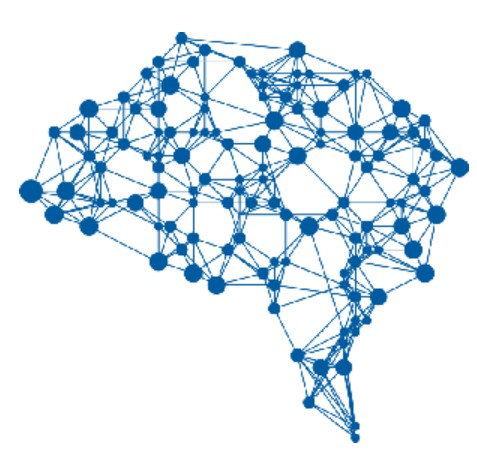
\includegraphics[scale=1]{0.DeepLearningLogo.jpg}
    \end{center}}



\begin{document}
\maketitle
\counterwithin{figure}{subsection}
\captionsetup[figure]{labelfont=bf}

\pagebreak

%% -- Sommario
\tableofcontents
\pagebreak


\section{Gradient Descent and Backpropagation}

\subsection{The Geometry of Optimization}
Once a neural network makes a prediction and calculates the error (Loss/Cost), it must adjust its weights to improve. The algorithm used to find the optimal weights is called \textbf{Gradient Descent}.

\begin{defbox}{Gradient Descent}
 Gradient Descent is an iterative optimization method used to minimize a function by moving the parameters step by step in the direction opposite to the gradient.
 \end{defbox}

To understand Gradient Descent, we must visualize the problem geometrically. Imagine the \textbf{Cost Function} as a physical landscape (a hypersurface) where the coordinates are the model's weights, and the elevation is the error.
\begin{itemize}
    \item \textbf{High elevation:} High error (bad predictions).
    \item \textbf{Low elevation (Valleys):} Low error (good predictions).
\end{itemize}

\begin{figure}[H] 
    \centering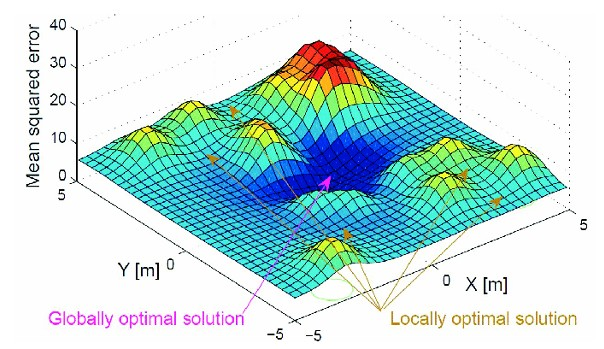
\includegraphics[scale=0.75]{12.The Cost Hypersuperface.jpg}
    \caption{The Cost Hypersuperface}
\captionsetup{font=footnotesize}
\end{figure}

 \begin{defbox}{Cost Hypersurface}
 A cost hypersurface is the geometric representation of the cost function in the parameter space of the model. Each point of this space corresponds to one specific configuration of the model parameters.
 \end{defbox}

\textbf{The Goal of Training:} To navigate the network's weights down the landscape until they reach the \textbf{Global Minimum} (the absolute lowest possible error).


 \begin{defbox}{Global Minimum}
 The global minimum is the absolute lowest point of the cost function over the entire parameter space.
 \end{defbox}

 \begin{defbox}{Local Minimum}
 A local minimum is a point whose cost is lower than that of nearby points, but not necessarily the lowest over the entire parameter space.
 \end{defbox}


\subsubsection{The Reality of the Loss Landscape.}
In simple models (like Linear Regression), this landscape is a smooth, bowl-shaped \textbf{Convex Function} with only one perfect bottom. 

 \begin{defbox}{Convex Function}
 A convex function is a function whose surface has only one global minimum and no local minima distinct from it.
 \end{defbox}

However, in Deep Learning (with millions of parameters), the landscape is highly \textbf{Non-Convex}. It is filled with jagged peaks, flat plateaus, and \textbf{Local Minima} (shallow valleys that trap the model before it reaches the true bottom). 

 \begin{defbox}{Non-Convex Function}
 A non-convex function is a function whose surface may contain many local minima, local maxima, saddle regions, and irregular shapes.
 \end{defbox}


\subsubsection{Different paths toward the minimum.}
The path followed during optimization depends on many factors. The goal is to find the weight configuration that minimizes the cost function, but convergence does not always happen in the same way.The speed of convergence depends on:
 \begin{itemize}
  \item the starting point,
  \item the shape of the cost surface,
  \item the step size used during exploration.
 \end{itemize}

The figure (\ref{fig13}) shows two different behaviors. In one case, the path is well-behaved and quickly reaches the minimum. In the other case, the path oscillates inside a narrow valley and converges more slowly.

\begin{figure}[H] 
    \centering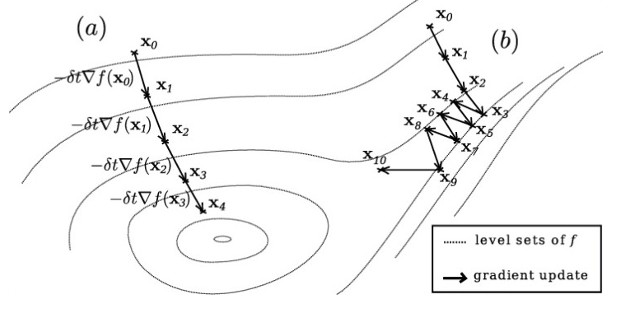
\includegraphics[scale=0.75]{13.Different path for the minimum.jpg}
    \caption{Different path for the minimum}
\captionsetup{font=footnotesize}
\label{fig13}
\end{figure}

This tells us that optimization is not only about the formula, but also about the geometry of the problem. A bad learning rate or a difficult landscape can make training unstable or slow.

 \begin{defbox}{Convergence}
 Convergence is the process through which an iterative optimization algorithm approaches a stable solution, ideally a minimum of the cost function.
 \end{defbox}

In practice, convergence means that after several updates the parameters are no longer changing significantly, and the cost function does not improve much anymore. 

Researchers use advanced projection techniques, like \textit{Filter Normalization}, to properly visualize these massive, chaotic multidimensional landscapes in 3D to understand how models learn.

\subsubsection{Visualizing the Loss Landscape: Filter Normalization}

Neural network loss landscapes exist in millions of dimensions. To visualize them, we plot a 2D slice as a 3D mountain range (where height = error). However, doing this naively creates a problem.

\begin{itemize}
    \item \textbf{The Problem (Scale Invariance):} In modern networks, you can scale weights up and down mathematically without changing the final prediction. 
    For example:
 \begin{itemize}
  \item we multiply the weights of one layer by a constant,
  \item and divide the weights of the following layer by the same constant.
 \end{itemize}
 Plotting these raw, unadjusted weights creates optical illusions, making smooth, easily trained valleys look like chaotic, jagged cliffs.
 \vs

    \item \textbf{The Solution (Filter Normalization):} To reveal the \textit{true} geometry of the landscape, we must scale our X and Y graphing axes to perfectly match the actual size (norm) of the model's filters. 
\end{itemize}

\subsubsection*{The 5-Step Visualization Process}
\begin{enumerate}
    \item \textbf{Center:} Start at the fully trained model's parameter vector ($\theta^*$).
    \item \textbf{Axes:} Pick two random direction vectors ($\delta$ and $\eta$) to act as your X and Y axes.
    \item \textbf{Normalize:} Rescale $\delta$ and $\eta$ so they match the scale of the model's filters.
    \item \textbf{Grid Evaluation:} Shift slightly around the center point and calculate the Loss across a 2D grid using the formula:
    $$ \theta = \theta^* + x\delta + y\eta $$
    \item \textbf{Plot:} Map these Loss values to the Z-axis (height) to create an accurate 3D surface map.
\end{enumerate}


 \begin{defbox}{Filter Normalization}
 Filter normalization is a visualization technique in which the directions used to explore the loss landscape are rescaled according to the norm of the model filters, so that the plotted surface is not distorted by scale invariance.
 \end{defbox}





\begin{figure}[H] 
    \centering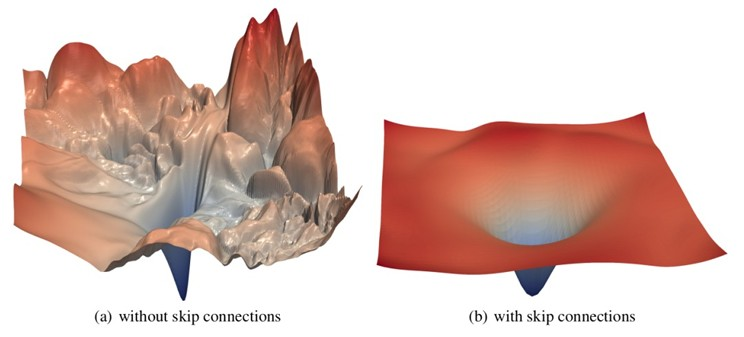
\includegraphics[scale=0.75]{14.Filter Normalization.jpg}
    \caption{Filter Normalization}
\captionsetup{font=footnotesize}
\end{figure}

In short, filter normalization helps us visualize the true shape of the loss landscape around the final trained model, avoiding misleading distortions caused by the scaling of the weights.

\subsection{The Mathematics of Gradient Descent}

We defined Gradient Descent as a numerical method used to find the minimum of a function of many variables. In this context, the function is the cost function \(C\), and the variables are the weights of the model.

 \begin{defbox}{Cost Function}
 The cost function is a function that measures how far the predictions of a model are from the desired targets over the training data.
 \end{defbox}

The cost is computed over the entire training dataset at each iteration.
We can write the approximate variation of the cost:
 \[
 \Delta C \sim \sum_{i=1}^{n} \frac{\partial C}{\partial w_i}\Delta w_i ,
 \]
where \(n\) is the number of weights.

This formula is the first-order approximation of how the cost changes when the weights are perturbed. It is a multivariable version of the linear approximation from calculus.

 \begin{defbox}{Partial Derivative}
 A partial derivative measures how a multivariable function changes when only one variable is varied while all the others are kept fixed.
 \end{defbox}

In optimization, the partial derivative \( \frac{\partial C}{\partial w_i} \) tells us how sensitive the cost is to changes in the weight \(w_i\). 

\vspace{-0.2cm}

\paragraph{ Link between \(\Delta C\) and \(\Delta w\).}
We can rewrites the previous expression using vector notation and introduces the gradient.

 \begin{defbox}{Gradient}
 The gradient of a function is the vector containing all its partial derivatives. It points in the direction of the greatest increase of the function.
 \end{defbox}

It is possible states that
 \[
 \Delta C \sim \nabla C \cdot \Delta w,
 \]
where
 \[
 \nabla C =
 \left(
 \frac{\partial C}{\partial w_1},
 \ldots,
 \frac{\partial C}{\partial w_n}
 \right)^T
 \]
is the gradient column vector, and \( \Delta w \) is the vector of weight variations.

The dot product \( \nabla C \cdot \Delta w \) tells us how the cost changes when we move in the direction \( \Delta w \). If we want the cost to decrease, we should choose \( \Delta w \) so that this dot product becomes negative. we introduce a small positive parameter $\eta$ and pose that:
 \[
 \Delta w = -\eta \nabla C,
 \]
where \( \eta > 0 \) is a small parameter. Substituting this into the previous formula gives:
 \begin{equation}
 \Delta C \sim -\eta \nabla C \cdot \nabla C = -\eta \|\nabla C\|^2.
 \end{equation}

Since \( \|\nabla C\|^2 \geq 0 \) and \( \eta > 0 \), we obtain \( \Delta C < 0 \) whenever the gradient is nonzero. This guarantees that, locally, the cost decreases.

 \begin{defbox}{Dot Product}
 The dot product between two vectors measures how much one vector points in the direction of the other.
 \end{defbox}

 \begin{defbox}{Learning Rate}
 The learning rate is a positive scalar that controls the size of the update step during optimization.
 \end{defbox}

This is the central mathematical intuition of Gradient Descent: move in the opposite direction of the gradient because that is the direction of the steepest local decrease. 



This gives us the fundamental \textbf{Weight Update Rule} of Machine Learning:
\begin{equation}
    w_{\text{new}} = w_{\text{old}} - \eta \nabla C
\end{equation}

My new weight equals my old weight, minus a small step in the direction that reduces the error.
\vspace{-0.2cm}

\paragraph*{The Danger of the Learning Rate ($\eta$).}
The Learning Rate is arguably the most important hyperparameter in Deep Learning. It dictates how large of a step the algorithm takes down the mountain and on the geometry of the cost function.

\begin{itemize}
    \item \textbf{If $\eta$ is too small:}  convergence may be very slow.
    \item \textbf{If $\eta$ is too large:}  the algorithm may overshoot the minimum and oscillate.
\end{itemize}



So the elegance of Gradient Descent lies in its simplicity, while its practical difficulty lies in choosing appropriate hyperparameters and handling difficult optimization landscapes. 


\subsubsection{When to Stop Training (Convergence vs. Overfitting)}
Training should not continue indefinitely. We monitor the Cost (Loss) Function during training to decide when to stop:
\begin{enumerate}
    \item \textbf{Convergence:} Stop when the loss function reaches a flat plateau and stops decreasing. The model has learned all it can.
    \item \textbf{Early Stopping (Preventing Overfitting):} We must monitor the loss on both the \textit{Training Set} and the \textit{Validation Set}. If the Training Loss continues to drop, but the Validation Loss starts to \textit{increase}, the model is \textbf{Overfitting} (memorizing the training data instead of learning general patterns). Training must be stopped immediately.
\end{enumerate}


\begin{figure}[H] 
    \centering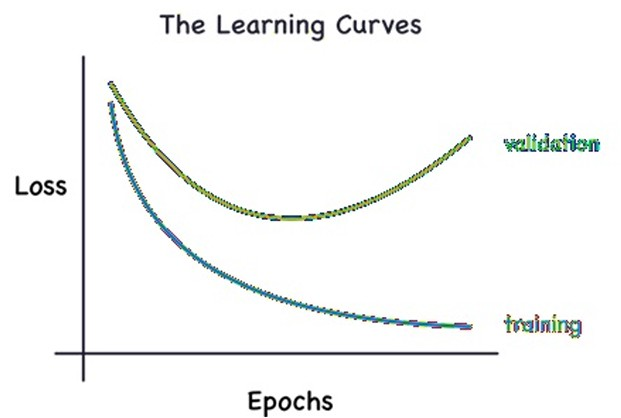
\includegraphics[scale=0.6]{15.Loss Validation vs Training set.jpg}
    \caption{Loss Validation vs Training set}
\captionsetup{font=footnotesize}
\end{figure}



In traditional data science, having too many dimensions (features) is bad: it causes data sparsity and increases compute time (The Curse of Dimensionality). 

However, in Deep Learning optimization, high dimensionality is actually a blessing. In a 3D landscape, it is easy to get stuck in a valley (Local Minimum) because there are only two directions to move (X and Y). In a 1-million-dimensional landscape, if 999,999 directions go uphill, there is almost certainly at least one direction that still goes downhill, allowing the algorithm to escape the trap and continue learning.

\subsection{Stochastic Gradient Descent (SGD)}
Standard Gradient Descent has a massive computational flaw: to take a \textit{single} step down the mountain, it must calculate the error across the \textit{entire} training dataset. If your dataset has 10 million images, computing 10 million errors before updating the weights once is too slow.

The solution is \textbf{Stochastic Gradient Descent (SGD)} using \textbf{Mini-Batches}.
Instead of looking at the whole dataset, SGD grabs a small, random handful of data (a mini-batch, e.g., 32 or 64 images). It calculates the gradient on just that small batch, and updates the weights immediately.

 \begin{defbox}{Stochastic Gradient Descent}
 Stochastic Gradient Descent (SGD) is an optimization method in which the gradient is estimated using only a small randomly selected subset of the training data instead of the entire dataset.
 \end{defbox}







\begin{itemize}
    \item \textbf{Trade-off:} The gradient calculated on a mini-batch is \textit{noisy} and imprecise compared to the exact gradient of the whole dataset. The path down the mountain will be jagged and zig-zagged.
    \item \textbf{Benefit:} Because it updates the weights instantly after just 32 images, the model trains exponentially faster.
\end{itemize}

\paragraph*{ Mini-batch update algorithm, batch, and epoch}

The practical algorithm used in mini-batch learning can be summerized like:



 \begin{itemize}
  \item \texttt{Step 1}: select \(m\) samples to form a mini-batch.

  \item \texttt{Step 2}: compute the gradient approximation on that mini-batch.
 
  \item \texttt{Step 3}: update the weights and biases using
  \[
  w'_k = w_k - \frac{\eta}{m}\sum_j \frac{\partial C_{x_j}}{\partial w_k},
  \qquad
  b'_l = b_l - \frac{\eta}{m}\sum_j \frac{\partial C_{x_j}}{\partial b_l}.
  \]
  \item \texttt{Step 4}: choose another random mini-batch and repeat the process.
  \item \texttt{Step 5}: continue until the entire training set has been processed.

  \item \texttt{Step 6}: repeat the whole process for multiple passes until convergence is reached.
 \end{itemize}


\subsubsection{Terminology of SGD}
\begin{itemize}
    \item \textbf{Mini-Batch:} The small subset of data used for a single weight update.
    \item \textbf{Iteration (or Step):} One update of the model's weights based on one mini-batch.
    \item \textbf{Epoch:} One complete pass through the \textit{entire} training dataset. (If your dataset has 1,000 images and your batch size is 100, it takes 10 iterations to complete 1 Epoch).
\end{itemize}




\subsection{Backpropation Method}
As established, \textbf{Backpropagation} calculates the gradient of the Loss function with respect to the network's weights and biases, allowing us to update them via Gradient Descent. 

Historically, backpropagation is a specific application of \textbf{Reverse-Mode Automatic Differentiation}. Popularized in 1986 by Rumelhart, Hinton, and Williams, it is the algorithm that single-handedly made the training of deep, multi-layer neural networks computationally feasible.

\subsubsection{The Computational Graph}
A neural network is best understood mathematically as a \textbf{Computational Graph}: a massive composite function broken down into a sequence of smaller, trackable operations. This allows us to split the training process into two phases:
\begin{enumerate}
    \item \textbf{Forward Phase:} The input flows left-to-right through the graph to compute the final prediction and the Loss.
    \item \textbf{Backward Phase:} The error flows right-to-left, using the Chain Rule to calculate gradients for every parameter.
\end{enumerate}


\begin{defbox}{Computational Graph}
A \textbf{computational graph} is a graph representation of a computation, where nodes correspond to operations or variables, and edges represent the flow of values between them.
\end{defbox}


\subsubsection{Standard Mathematical Notation}
To perform backpropagation on a large scale, we must use precise notation. Let $l$ denote the current layer, and $l-1$ the previous layer. 

The calculation for a layer is split into two distinct variables: the linear \textbf{Weighted Input} ($z$) and the non-linear \textbf{Activation} ($a$).

\vspace{-0.2cm}
\paragraph*{1. The Weighted Input ($z$).}
Before applying the activation function, we calculate the raw linear combination of the previous layer's outputs. For a single neuron $j$ in layer $l$:
\begin{equation}
    z_j^l = \sum_k w_{jk}^{l} a_k^{l-1} + b_j^l
\end{equation}
In compact vector/matrix notation for the entire layer:
\begin{equation}
    \mathbf{z}^{l} = (\mathbf{W}^{l})^{T} \mathbf{a}^{l-1} + \mathbf{b}^{l}
\end{equation}

\vspace{-0.2cm}
\paragraph*{2. The Activation ($a$)}
We then apply the non-linear activation function ($\sigma$) element-wise to the weighted input:
\begin{equation}
    \mathbf{a}^{l} = \sigma(\mathbf{z}^{l})
\end{equation}
\textit{Why separate them?} During the backward phase, we will need to calculate the derivative of the activation function with respect to its input. Explicitly defining $\mathbf{z}^{l}$ makes calculating $\frac{\partial \mathbf{a}}{\partial \mathbf{z}}$ mathematically cleaner.

\begin{defbox}{Activation of a Neuron}
The \textbf{activation} of a neuron is the output value produced by applying the activation function to the weighted sum of the inputs plus the bias.
\end{defbox}

\subsubsection{The Two Assumptions of the Cost (Loss) Function}
For the backpropagation algorithm to work, the chosen Cost Function ($C$) must strictly satisfy two mathematical assumptions:

\begin{enumerate}
\item \textbf{It must be an average of individual examples}


The total cost must be the average of the costs calculated for individual training examples ($x$):
\begin{equation*}
    C = \frac{1}{n} \sum_x C_x
\end{equation*}
\textit{Why?} This allows the algorithm to calculate the gradient for a single training example ($C_x$) first, and then average the gradients across a batch of data.

\vspace{0.25cm}
\item \textbf{ It must be a function of the network's output}

The cost must be calculable using only the target labels and the final activation vector of the output layer ($a^L$).
\textit{Why?} Because backpropagation applies the Chain Rule starting from the very end of the network. If the cost function did not explicitly depend on the final output $a^L$, we could not calculate the first required derivative ($\frac{\partial C}{\partial a^L}$).
\end{enumerate}

\vs
\begin{example}{\textbf{The Quadratic Cost Function (MSE)}}

The classic Mean Squared Error (MSE) function perfectly satisfies both assumptions. 
\begin{equation}
    C = \frac{1}{2n}\sum_x \left\| y(x) - a^L(x) \right\|^2
\end{equation}
\begin{itemize}
    \item It satisfies Assumption 1 because the $\sum_x$ averages the errors over $n$ examples.
    \item It satisfies Assumption 2 because the error is directly calculated using $a^L(x)$, the network's final output.
\end{itemize}
\end{example}

\subsection{The Four Fundamental Equations of Backpropagation}

\subsubsection{The Concept of "Neuron Error" ($\delta$)}
To compute the gradients efficiently without doing redundant calculus for every single parameter, backpropagation introduces an intermediate variable called the \textbf{Neuron Error}, denoted by $\delta_j^l$ (the error of neuron $j$ in layer $l$).

Mathematically, it is the partial derivative of the Cost function with respect to the neuron's \textit{weighted input} ($z$):
\[ \delta_j^l = \frac{\partial C}{\partial z_j^l} \]

If this error term is large, changing the neuron's input will drastically change the final cost. If it is close to zero, the neuron is already optimized (or saturated). The entire backpropagation algorithm is simply the process of calculating this $\delta$ for the output layer, passing it backwards, and using it to update the weights and biases.

\subsubsection{BP1: Error in the Output Layer}
The first step is to calculate the error at the very end of the network (Layer $L$).
\[ \delta^L = \nabla_{a^L} C \odot \sigma'(z^L) \]

\textbf{What it means:} 
The error in the output layer is the product of two things:
\begin{enumerate}
    \item $\nabla_{a^L} C$: How fast the cost changes with respect to the final prediction (e.g., Prediction minus True Target).
    \item $\sigma'(z^L)$: The slope of the activation function.
\end{enumerate}
The symbol $\odot$ represents the \textbf{Hadamard Product} (element-wise multiplication).

\subsubsection{BP2: Propagating the Error Backward (Hidden Layers)}
Once we have the error at the output layer, we calculate the error for the hidden layer immediately before it, and so on, moving backwards.
\[ \delta^l = \left((W^{l+1})^T \delta^{l+1}\right) \odot \sigma'(z^l) \]

\textbf{What it means:} 
You do not need to recalculate the error from scratch. You take the error from the \textit{next} layer ($\delta^{l+1}$), pull it backwards through the weights connecting them ($(W^{l+1})^T$), and multiply it by the slope of the current layer's activation function ($\sigma'(z^l)$). This is the exact mechanism that allows deep networks to train efficiently.

\subsubsection{BP3: Derivative of the Cost with Respect to Biases}
Once the neuron error ($\delta$) is calculated for a layer, finding the gradient for the biases is trivial.
\[ \frac{\partial C}{\partial b_j^l} = \delta_j^l \]

\textbf{What it means:} 
The gradient of the bias is exactly equal to the neuron's error. If a neuron has a large error, its bias gets updated by a large amount.

\subsubsection{BP4: Derivative of the Cost with Respect to Weights}
This is the most important equation for understanding how networks learn.
\[ \frac{\partial C}{\partial w_{jk}^l} = a_k^{l-1} \cdot \delta_j^l \]

\textbf{What it means:} 
The gradient for any given weight is simply:
\[ \text{Gradient} = \text{Incoming Activation } (a_{\text{in}}) \times \text{Outgoing Error } (\delta_{\text{out}}) \]
If the incoming signal to a weight is strong, and the resulting error of the neuron it connects to is large, the weight is heavily responsible for the mistake and will receive a massive update.

\subsubsection{The Complete Algorithm Summary}
To train a neural network, these four equations are executed in a strict loop:
\begin{enumerate}
    \item \textbf{Forward Pass:} Compute all weighted inputs ($z$) and activations ($a$) until you get a prediction.
    \item \textbf{Output Error (BP1):} Calculate $\delta^L$ at the final layer.
    \item \textbf{Backpropagate Error (BP2):} Pass the $\delta$ backwards to compute the error for all hidden layers.
    \item \textbf{Calculate Gradients (BP3 \& BP4):} Use the $\delta$ terms to instantly calculate the gradients for every single bias and weight in the network.
    \item \textbf{Gradient Descent:} Update the parameters and repeat.
\end{enumerate}

\subsection{Implications of Backpropagation: Learning Dynamics and Bottlenecks}

\subsubsection{Learning Speed and Gradient Magnitude}
The equations of Backpropagation (specifically BP4) dictate how fast a network learns.
\[ \frac{\partial C}{\partial w_{jk}^l} = a_k^{l-1} \cdot \delta_j^l \]

This equation reveals a harsh truth about Gradient Descent: \textbf{The speed at which a parameter learns is directly proportional to the magnitude of its gradient.} If either the incoming activation ($a_{\text{in}}$) or the neuron error ($\delta_{\text{out}}$) is very small, the resulting gradient is tiny. A tiny gradient means a microscopic weight update, causing the network to learn painfully slowly.

\subsubsection{The Saturation Problem}
Look at the formula for the output error (BP1): 
\[ \delta^L = \nabla_{a^L} C \odot \sigma'(z^L) \]

The gradient is multiplied by the derivative of the activation function ($\sigma'$). If you use a Sigmoid function, its values are squeezed between 0 and 1. 
\begin{itemize}
    \item If the neuron is highly active (output near 1) or highly inactive (output near 0), the curve becomes completely flat.
    \item A flat curve has a slope (derivative) of roughly $0$.
\end{itemize}
When this happens, the neuron is said to be \textbf{saturated}. Because $\sigma'(z) \approx 0$, the entire $\delta$ term becomes $0$. The error signal is \textit{killed,} and the weights connected to that neuron stop updating. \textit{Data Science Takeaway:} This is the exact reason why modern Deep Learning rarely uses Sigmoid for hidden layers, opting for ReLU instead.

\subsubsection{The Vanishing Gradient Problem in Deep Networks}
The saturation problem compounds geometrically as you build deeper networks. 

According to BP2, the error is passed backwards layer by layer, multiplying by the activation derivative ($\sigma'$) at each step. Because the derivative of a Sigmoid is always less than 0.25, you are repeatedly multiplying by fractions:
\[ \delta \times 0.2 \times 0.1 \times 0.2 \dots \]

By the time the error signal reaches the very first hidden layers of a deep network, the gradient has shrunk to microscopic levels (e.g., $10^{-15}$). This is the \textbf{Vanishing Gradient Problem}. The early layers of the network, which are responsible for learning foundational features, receive almost no learning signal and fail to train.

\subsubsection{The Complete Training Loop (Stochastic Gradient Descent)}
 backpropagation alone does not update the weights. It only computes the gradients. To actually learn, it must be combined with an optimization method. To train a model, we combine it with \textbf{Stochastic Gradient Descent (SGD)} using \textbf{Mini-Batches} and \textbf{Epochs}.

\begin{enumerate}
    \item \textbf{Mini-Batch Selection:} Select a small subset of the training data (e.g., 32 images).
    \item \textbf{Forward Pass:} Pass all 32 images through the network to calculate predictions.
    \item \textbf{Calculate Error:} Compute the loss and apply BP1 for the output layer.
    \item \textbf{Backpropagate:} Apply BP2 to push the error backwards through the hidden layers.
    \item \textbf{Calculate Gradients:} Apply BP3 and BP4 to find the gradients for all weights and biases.
    \item \textbf{Average and Update:} Average the 32 gradients together, multiply by the learning rate ($\eta$), and update the actual weights.
    \item \textbf{Next Batch:} Move to the next batch until the entire dataset has been seen. This completes one \textbf{Epoch}.
\end{enumerate}


\pagebreak

\end{document}